\subsection{Motivation}
\begin{frame} %%Eine Folie
  	\frametitle{Motivation}
  	\begin{center}
  	\small Technologieübersicht verschiedener Tracking-Methoden.
  	\end{center}
%
	\begin{table} [H]
		\begin{center}
			\begin{tabular}{rllll}
				\textbf{Arbeitsweise} & \textbf{Optisch} & \textbf{Magnetisch} & \textbf{Ultraschall} & \textbf{ Funk (UHF)} \\
				\textbf{Genauigkeit} & gut & ausreichend & gut & sehr gut \\
				\textbf{Frequenz} & mittel & hoch & gering & hoch \\
				\textbf{Volumen} & mittel & klein & mittel & groß \\
				\textbf{LOS} & Ja & Ja & Nein & Nein \\
				\textbf{In Vivo} & Nein   & Nein & Nein & Ja \\
%			
			\end{tabular}
		\end{center}
%		\caption[Übersicht Navigationsverfahren]{Grobe Übersicht und Einteilung verschiedener Navigationsverfahren anhand ihres physikalischen Messprinzips.}
		\label{tab:overview_tracking}
	\end{table}  	
\end{frame}
%------------------------------------------------------
\begin{frame}{Graphics} 
	\frametitle{Mathematische Grundlagen I }
	\centering
	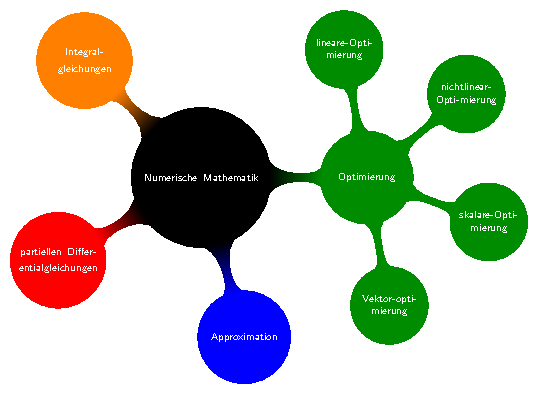
\includegraphics[page=1, width=.6\textwidth]{../img/mindmap.pdf}\\
%--
	\tiny Evolutionäre Verfahren sind Teilgebiet der \textbf{nichtlinearen Optimierung}
\end{frame}
%------------------------------------------------------
\begin{frame}{Graphics} 
  	\frametitle{Mathematische Grundlagen II}
	\includegraphics[page=1, width=.6\textwidth]{../img/FlowChart_EvolutionaryOptimization.pdf}
\end{frame}
%------------------------------------------------------
\begin{frame}{Graphics} 
  	\frametitle{Mathematische Grundlagen III}
%  	
  	\begin{textblock*}{6cm}(6cm,2cm) % {block width} (coords)
  		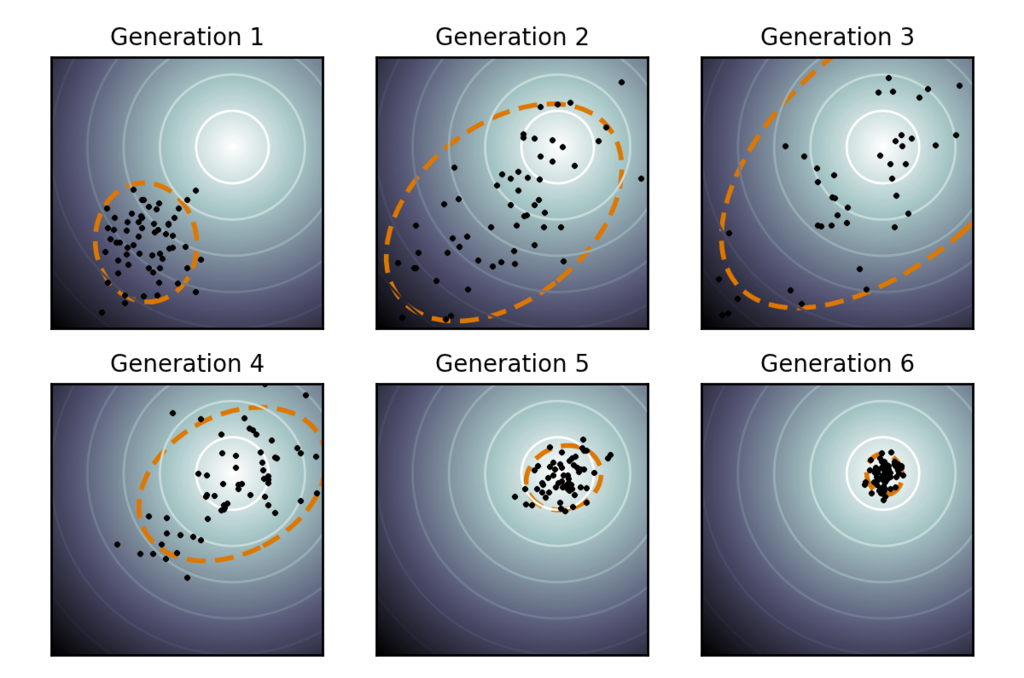
\includegraphics[width=6cm]{../img/Concept_of_directional_optimization_in_CMA-ES_algorithm.png}
  	\end{textblock*}
%  	
  	\footnote{Grafik entnommen aus \url{http://en.wikipedia.org/w/index.php?title=File:Concept_of_directional_optimization_in_CMA-ES_algorithm.png&oldid=532567533}}
%  	
\end{frame}
%------------------------------------------------------
\subsection{Grundlagen}
\begin{frame} %%Eine Folie
  \frametitle{Beispiel}
  \movie[options]{placeholder box}{../vid/vid1.avi}
\end{frame}
%------------------------------------------------------
\begin{frame}
  \frametitle{Physikalische Grundlagen}
	- Funk basierende Messung auf dem RFID-Standard 
	- Phasenmessung
\end{frame}
%------------------------------------------------------
%\subsection{Grundlagen2}
%\begin{frame}
%  \frametitle{Test}
%  \begin{fazit} %%Definition
%    Beschreibung des Problems
%  \end{fazit}
%\end{frame}
